\chapter{Experiments}
\ifpdf
    \graphicspath{{Chapter3/Chapter3Figs/PNG/}{Chapter3/Chapter3Figs/PDF/}{Chapter3/Chapter3Figs/}}
\else
    \graphicspath{{Chapter3/Chapter3Figs/EPS/}{Chapter3/Chapter3Figs/}}
\fi

\section{CheXpert Dataset}

The CheXpert (\cite{irvin2019chexpert}) dataset contains 224,316 chest radiographs of 65,240 patients with both frontal and lateral views available. This dataset was created to perform automated chest x-ray interpretation, featuring uncertainty labels and radiologist-labeled reference standard evaluation sets. This is a multi-label dataset containing 14 chest disease labels that can be detected using x-ray images. A multi-label dataset is a dataset which has more than one output class with label 1 for a given input. In this context, a patient can have more than one disease which is reflected in the dataset as well. Some images are of 320 x 320 and some are of 390 x 320. This dataset has both frontal and lateral views. However, we have reduced the image size in our training setup to 224 x 224 in order to match the input shape of the neural network model.

The performance of the model trained on CheXpert is evaluated using the provided validation set which has 200 images. However, the validation set has only 5 disease labels. So, we have considered only 5 corresponding disease labels for training to maintain consistency. The diseases considered are  Atelectasis, Cardiomegaly, Consolidation, Edema and Pleural Effusion. Every disease has 3 labels: either 0(negative), 1(positive), -1(uncertain). There are various ways to handle the uncertain labels as shown in \cite{irvin2019chexpert}. We have assigned label 1 to Cardiomegaly and Edema and label 0 to the rest 3 diseases as it has been empirically found that this way of modifying uncertain labels has shown the most appropriate results. 

\section{Metrics}

\subsection{AUC}

\begin{figure}[!htbp]
  \begin{center}
    \leavevmode
    \ifpdf
      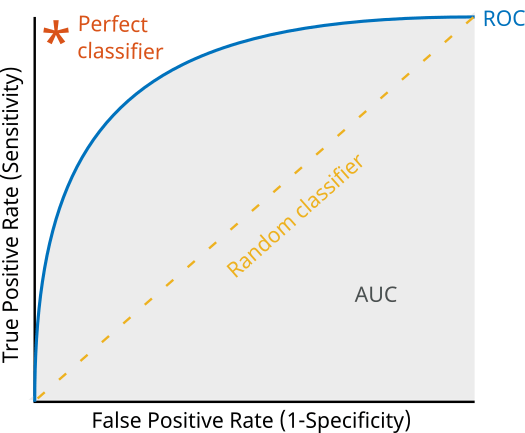
\includegraphics[scale=0.4]
      {Chapter3/Chapter3Figs/AUC.png}    
    \fi
    \caption{AUC (Area under the ROC Curve)}
    \label{auc}
  \end{center}
\end{figure}

AUC stands for Area under the ROC Curve. An ROC curve (receiver operating characteristic curve) is a graph showing the performance of a classification model at all classification thresholds. This curve plots two parameters: True Positive Rate (TPR) and False Positive Rate (FPR). True Positive Rate is the probability that an actual positive sample is classified as positive. False Positive Rate is the probability that an actual negative sample is misclassified as positive. An ROC curve plots TPR vs. FPR at different classification thresholds. AUC measures the entire two-dimensional area underneath the entire ROC curve from (0,0) to (1,1). Higher the AUC value, better the model performance. 



\subsection{Expected Calibration Error}

Expected Calibration Error quantifies how well a given model is calibrated i.e how well the predicted output probabilities of the model matches the actual probabilities of the ground truth distribution. Expected Calibration Error was introduced by \cite{naeini2015obtaining}. In computing ECE, the predictions are sorted and partitioned into N fixed number of bins (N = 15 in our experiments). The predicted value of
each test instance falls into one of the bins. The ECE calculates Expected Calibration Error over the bins. The formula of Expected Calibration Error is given as:

\begin{center}
{ $ECE=\sum_{i=1}^Nb_i||p_i-c_i||$}
\end{center}


\section{Evaluation of baseline methods and modified pipeline}

\begin{table}[htbp]
\centering
\begin{tabular}{|p{1.5cm}|p{2.25cm}|p{2.25cm}|p{2.25cm}|p{1.5cm}|p{2.25cm}|p{1.25cm}|}
  \hline
  Loss & Atelectasis & Cardiomegaly & Consolidation & Edema & Pleural Effusion & Mean\\
  \hline
  Cross Entropy  &  0.769 &
0.764 &
0.751 &
0.675 &
0.822 &
0.756
\\
  \hline  
  Custom &  0.722 &
0.807 &
0.743 &
0.645 &
0.806 &
0.745

\\
  \hline
  Modified Pipeline &  0.752 &
0.810 &
0.716 &
0.646 &
0.822 &
0.749

\\
  \hline
\end{tabular}
\caption{\label{baseline_results}Table Showing Performance Comparison (Validation AUC values) on model trained on 15 epochs of Cross Entropy Loss, Class Distinctiveness Paired with Cross Entropy and the Double Stage Pipeline with Class Distinctiveness and Cross Entropy Losses}
\end{table}

We perform an ablation study on the baseline loss functions introduced in \cite{MAHAPATRA2022102551}. 
We trained and validated the DenseNet121 model only with the crossentropy loss and the crossentropy loss coupled with the class distinctiveness loss. We don't present here the results when the spatial coherence loss is considered, as the model training takes too much time when the spatial coherence loss is incorporated and it doesn't seem to converge within reasonable time limits. 

For the cross entropy loss with the class distinctiveness loss, we try two approaches. First, training the model from random initial weights with both the loss terms. Second, training the model first only on the weighted cross entropy followed by further training the model on the modified loss term with class distinctiveness loss. The results of all the three approaches when trained and validated on 15 epochs is as shown in Table \ref{baseline_results}.

The two stage training schedule is expected to perform better and achieve faster convergence because of the concern of the model diverging if classdistinctiveness is used at the beginning with \textbf{bad  saliency maps}, i.e. model not good enough to get relevant saliency maps.
The best AUC from Table \ref{baseline_results} seem to appear from the Cross Entropy loss only, followed by the custom loss using the double stage modified pipeline and followed by the standard custom loss, single stage pipeline.

\begin{figure}[!htbp]
  \begin{center}
    \leavevmode
    \ifpdf
      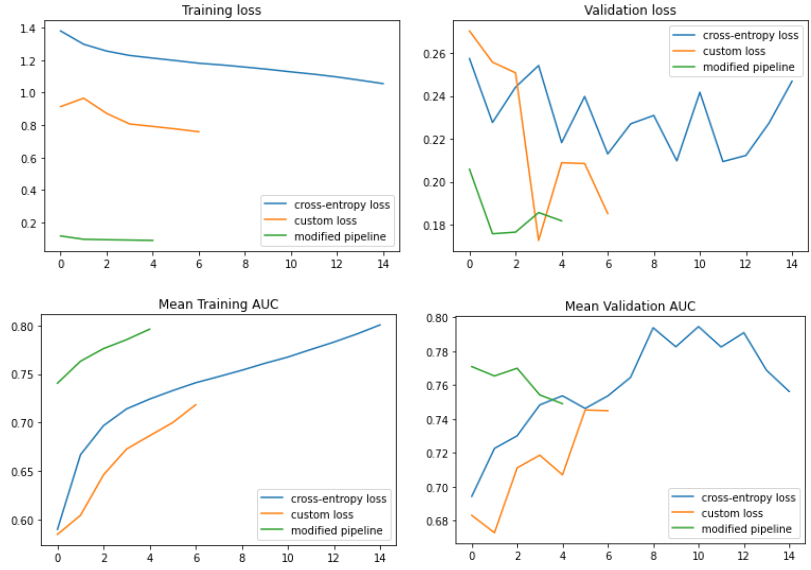
\includegraphics[scale=0.5]
      {Chapter3/Chapter3Figs/baseline_gs.png}    
    \fi
    \caption{Plots showing the training and validation loss and auc vary with number of epochs}
    \label{baseline_res}
  \end{center}
\end{figure}
When experimenting with custom loss using class distinctiveness loss, we do grid search for the hyperparameter $\lambda_1$, to get optimal value almost 1.4 as suggested in the paper.

\section{Debugging Class Distinctiveness Loss}
Class distinctiveness loss, does one thing well, it makes sure the saliency maps corresponding to different maps look reasonably different. But it doesn't necessarily give maps close to the reality. Not knowing the ground truth makes for the model hard to converge.
 Other hyperparameters like $\lambda_1$, learning rate and drop out rate were changed to obtain optimal ones. Still finally the custom loss usually achieved performance atmost as good as the cross-entropy loss.
 \begin{figure}
  \centering
  \begin{minipage}[b]{0.45\textwidth}
    \centering
    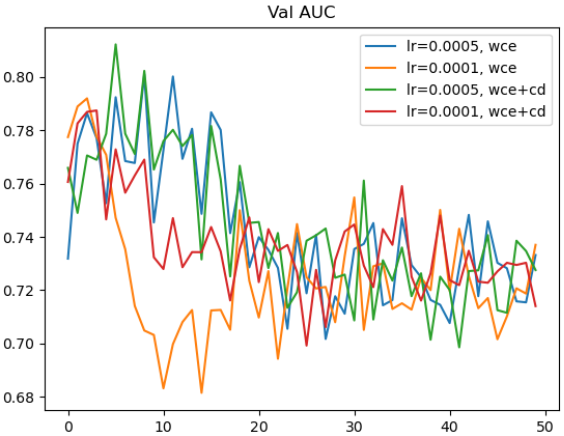
\includegraphics[width=\textwidth]{Chapter3/Chapter3Figs/lr.png}
    \caption{Graph showing val AUC vs number of epochs for model trained for 50 epochs for different learning rates}
    \label{fig:lr}
  \end{minipage}
  \hfill
  \begin{minipage}[b]{0.45\textwidth}
    \centering
    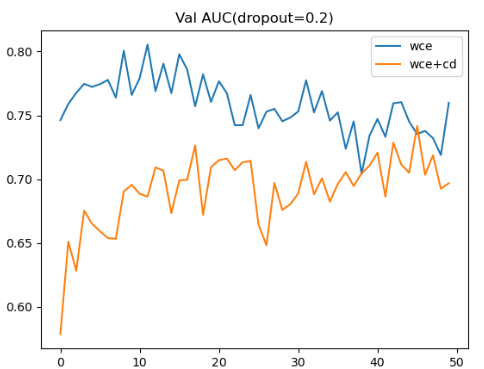
\includegraphics[width=\textwidth]{Chapter3/Chapter3Figs/drop.png}
    \caption{Graph showing val AUC vs number of epochs for model trained for 50 epochs for different dropout rates}
    \label{fig:drop}
  \end{minipage}
\end{figure}
\section{Experiments with Different Architectures}
We also experimented with 3 different backbone networks with other factors same. Namely we used the Densenet-121, Resnet-101 and VGG-19 as our model backbones
All the three backbone based methods, after 15 epochs obtained AUCs of over 0.8. The saliency maps corresponding to the three methods, are plotted in \ref{sal_diff_loss}.
\begin{figure}[!htbp]
  \begin{center}
    \leavevmode
    \ifpdf
      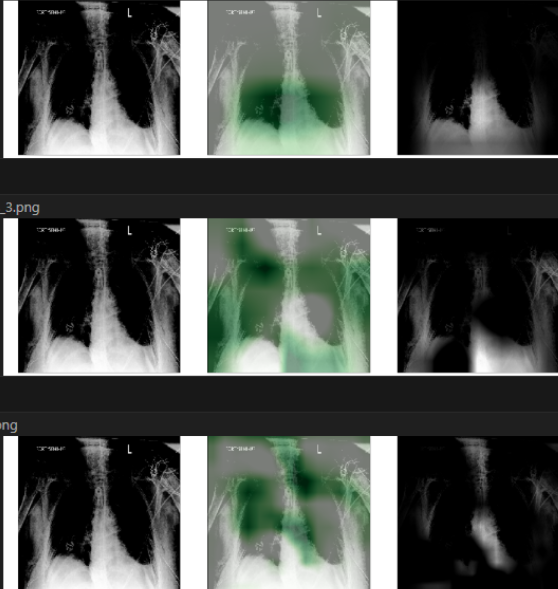
\includegraphics[scale=0.6]
      {Chapter3/Chapter3Figs/sal_arch}    
    \fi
    \caption{Saliency Maps for models trained with different backbone networks, top row for Cross Entropy Loss, middle row for Resnet101, and third VGG-19}
    \label{sal_diff_loss}
  \end{center}
\end{figure}
\section{Experiments with newly introduced loss functions}

\begin{table}[htbp]
\centering
\begin{tabular}{|p{1.8cm}|p{1.9cm}|p{2.4cm}|p{2.4cm}|p{1.3cm}|p{1.5cm}|p{1.1cm}|}
  \hline
   Loss Function & Atelectasis & Cardiomegaly & Consolidation & Edema & Pleural Effusion & Mean \\
  \hline
  Cross Entropy Loss &  0.8350 & 0.9032 & 0.9120 & 0.8489 & 0.9217 & 0.8841 \\
  \hline  
  Focal Loss & 0.8568 & 0.9077 & 0.9016 & 0.8447 & 0.9230 & 0.8867 \\
  \hline
  DeepAUC Loss & 0.7368 & 0.8263 & 0.9160 & 0.8269 & 0.8393 & 0.8291 \\
  \hline
\end{tabular}
\caption{\label{diffloss} Performance comparison (Validation AUC) across different loss functions}
\end{table}

\begin{figure}[!htbp]
  \begin{center}
    \leavevmode
    \ifpdf
      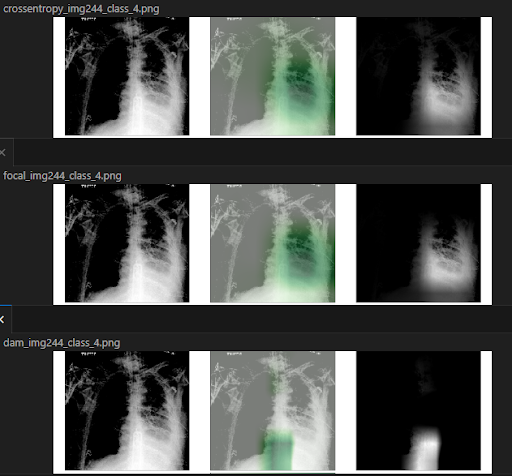
\includegraphics[scale=0.6]
      {Chapter3/Chapter3Figs/sal_diff_loss.png}    
    \fi
    \caption{Saliency Maps for all 3 models trained with different loss functions over an image.}
    \label{sal_diff_loss}
  \end{center}
\end{figure}

As we introduced Focal Loss and Deep AUC Maximization, we trained our DenseNet121 model on CheXpert dataset to analyse its performance under different loss functions. We used Adam Optimizer with a learning rate of 1e-4 and weight decay of 1e-5. We fixed the batch size of training data as 64 and trained our model for 5 epochs across all loss functions. One more interesting thing to note here is that we were able to improve the performance of model trained with Cross Entropy Loss from just 0.80 AUC to 0.88 AUC by finding and utilizing better hyperparameters. 

The results obtained are displayed in the table \ref{diffloss}. We can observe that Focal Loss has performed marginally better than Cross Entropy Loss. DeepAUC Loss, however, is not able to match the performance of other two loss functions, despite its objective being maximizing the very metric that is used to evaluate the model. 

In addition, we have also obtained the saliency maps of the models trained with these loss functions over a sample image as shown in figure \ref{sal_diff_loss}. The top, middle and bottom rows denote Cross Entropy Loss, Focal Loss and Deep AUC Loss. The left column denotes the input image and the next two columns display the obtained saliency maps denoting the regions learnt by the model pertaining to certain class. Here, we have obtained the region pertaining to class 4 for different models. We can observe that the saliency maps obtained for Cross Entropy Loss and Focal Loss are almost identical. We can probably attribute that to the fact that the mathematical form of Cross Entropy Loss and Focal Loss are almost identical, thus they learnt in an almost identical manner. It could also be possible that the both models have learnt well for the particular class and thus generated identical saliency maps. The saliency map obtained for DeepAUC Loss looks different when compared to the other two loss functions. As displayed in table \ref{diffloss}, DeepAUC Loss is less accurate than the other two loss functions, so probably the saliency map generated DeepAUC Loss is not accurate. However, we don't have any way to verify our findings and hypotheses due to lack of domain knowledge i.e the ability to diagnose diseases using chest x-rays in this context. Therefore, we can't perform qualitative analysis of saliency maps with certainty. 

\section{Calibration of the trained models}

\begin{table}[htbp]
\centering
\begin{tabular}{|p{1.8cm}|p{3.2cm}|p{3.2cm}|}
  \hline
   Loss Function & Mean ECE before calibration & Mean ECE after calibration \\
  \hline
  Cross Entropy Loss & 0.1147 & 0.0996 \\
  \hline  
  Focal Loss & 0.1763 & 0.1091 \\
  \hline
  DeepAUC Loss & 0.2348 & 0.0992 \\
  \hline
\end{tabular}
\caption{\label{ece} Mean ECE before and after calibrating the model using Temperature Scaling}
\end{table}

We calibrated the models trained under 3 different loss functions using Temperature Scaling. We have compared the calibration errors obtained before and after calibration for all 3 loss function in table \ref{ece}. We can observe that in all 3 cases, the mean ECE has reduced after calibration. We can also observe that the model trained with Cross Entropy Loss is the most calibrated model which means that the predictions of the model are closer to the ground truth distribtion and thus more reliable, even though the model trained with Focal Loss obtained marginally better AUC. Therefore, the model trained with Cross Entropy Loss is the most reliable model and the model performance is almost as good as the best one. After calibration though, all 3 models have similar mean ECE values. So after calibration, all 3 models are equally reliable. The drop in ECE value after calibration, especially in the case of DeepAUC Loss which is around 0.1356, shows that calibration is a very important step after the model training is completed to improve the reliability of the model which is very important in critical medical applications. 

% ------------------------------------------------------------------------


%%% Local Variables: 
%%% mode: latex
%%% TeX-master: "../thesis"
%%% End: 
